% \documentclass[a4paper, technote, draft, compsoc]{IEEEtran}
\documentclass[a4paper, technote,compsoc]{IEEEtran}
%\documentclass[a4paper]{article}

\usepackage[toc,page,titletoc]{appendix}
\usepackage[T1]{fontenc}    % use 8-bit T1 fonts
\usepackage[utf8]{inputenc} % allow utf-8 input
\usepackage{amsmath}
% \usepackage{hyperref}
\usepackage{amssymb}
\usepackage{booktabs}
\usepackage{multirow}
\usepackage{float}  % used to fix location of images i.e.\begin{figure}[H]
\usepackage{graphicx}  %needed to include png, eps figures
\usepackage{mwe}
\usepackage{url} % correct bad hyphenation here
\usepackage[dvipsnames]{xcolor}
% \usepackage{todonotes}
\usepackage{xr}
\usepackage{subfiles}
\usepackage{physics}
\usepackage{epigraph}
\usepackage{pdfpages}
% \usepackage{savetrees}

\usepackage{todonotes,tocloft,xpatch,hyperref}
\hypersetup{
    colorlinks,
    linkcolor={red!50!black},
    citecolor={blue!50!black},
    urlcolor={blue!80!black}
}

% This is based on classicthesis chapter definition
\let\oldsec=\section
\renewcommand*{\section}{\secdef{\Sec}{\SecS}}
\newcommand\SecS[1]{\oldsec*{#1}}%
\newcommand\Sec[2][]{\oldsec[\texorpdfstring{#1}{#1}]{#2}}%

% https://tex.stackexchange.com/a/61267/11984
\makeatletter
\xapptocmd{\Sec}{\addtocontents{tdo}{\protect\todoline{\thesection}{#1}{}}}{}{}
\newcommand{\todoline}[1]{\@ifnextchar\Endoftdo{}{\@todoline{#1}}}
\newcommand{\@todoline}[3]{%
  \@ifnextchar\todoline
    {}
    {\contentsline{section}{\numberline{#1}#2}{#3}{}{}}%
}
\let\l@todo\l@subsection
\newcommand{\Endoftdo}{}

\AtEndDocument{\addtocontents{tdo}{\string\Endoftdo}}
\makeatother


\externaldocument[M-]{main}

\usepackage[style=ieee]{biblatex}
\bibliography{xampl}
% \usepackage[backend=biber,style=ieee]{biblatex} 
\bibliography{bibliography.bib} %your file created using JabRef

% https://tex.stackexchange.com/questions/246/when-should-i-use-input-vs-include
% \newcommand{\N}{\mathbb{N}}
\newcommand{\Z}{\mathbb{Z}}
\newcommand{\Q}{\mathbb{Q}}

\newcommand{\R}{\mathbb{R}}
\newcommand{\RR}{\mathbb{R}^2}
\newcommand{\RRR}{\mathbb{R}^3}

\renewcommand{\Pmu}{\mathcal{P}}
\renewcommand{\P}{\mathbb{P}}

\newcommand{\delt}{\Delta t}
\newcommand{\utk}{{\widetilde u}^k}
\newcommand{\ut}[1]{{\widetilde u}^{#1}}
\newcommand{\rhog}{\text{\boldmath{$\rho$}}}
\renewcommand{\eps}{\varepsilon}

\DeclareMathOperator{\sspn}{span}
\newcommand{\spn}[1]{\sspn\left(#1\right)}
\newcommand{\mytodo}[1]{\todo[inline, color=green!20, inlinewidth=\columnwidth]{#1}}

\begin{document}

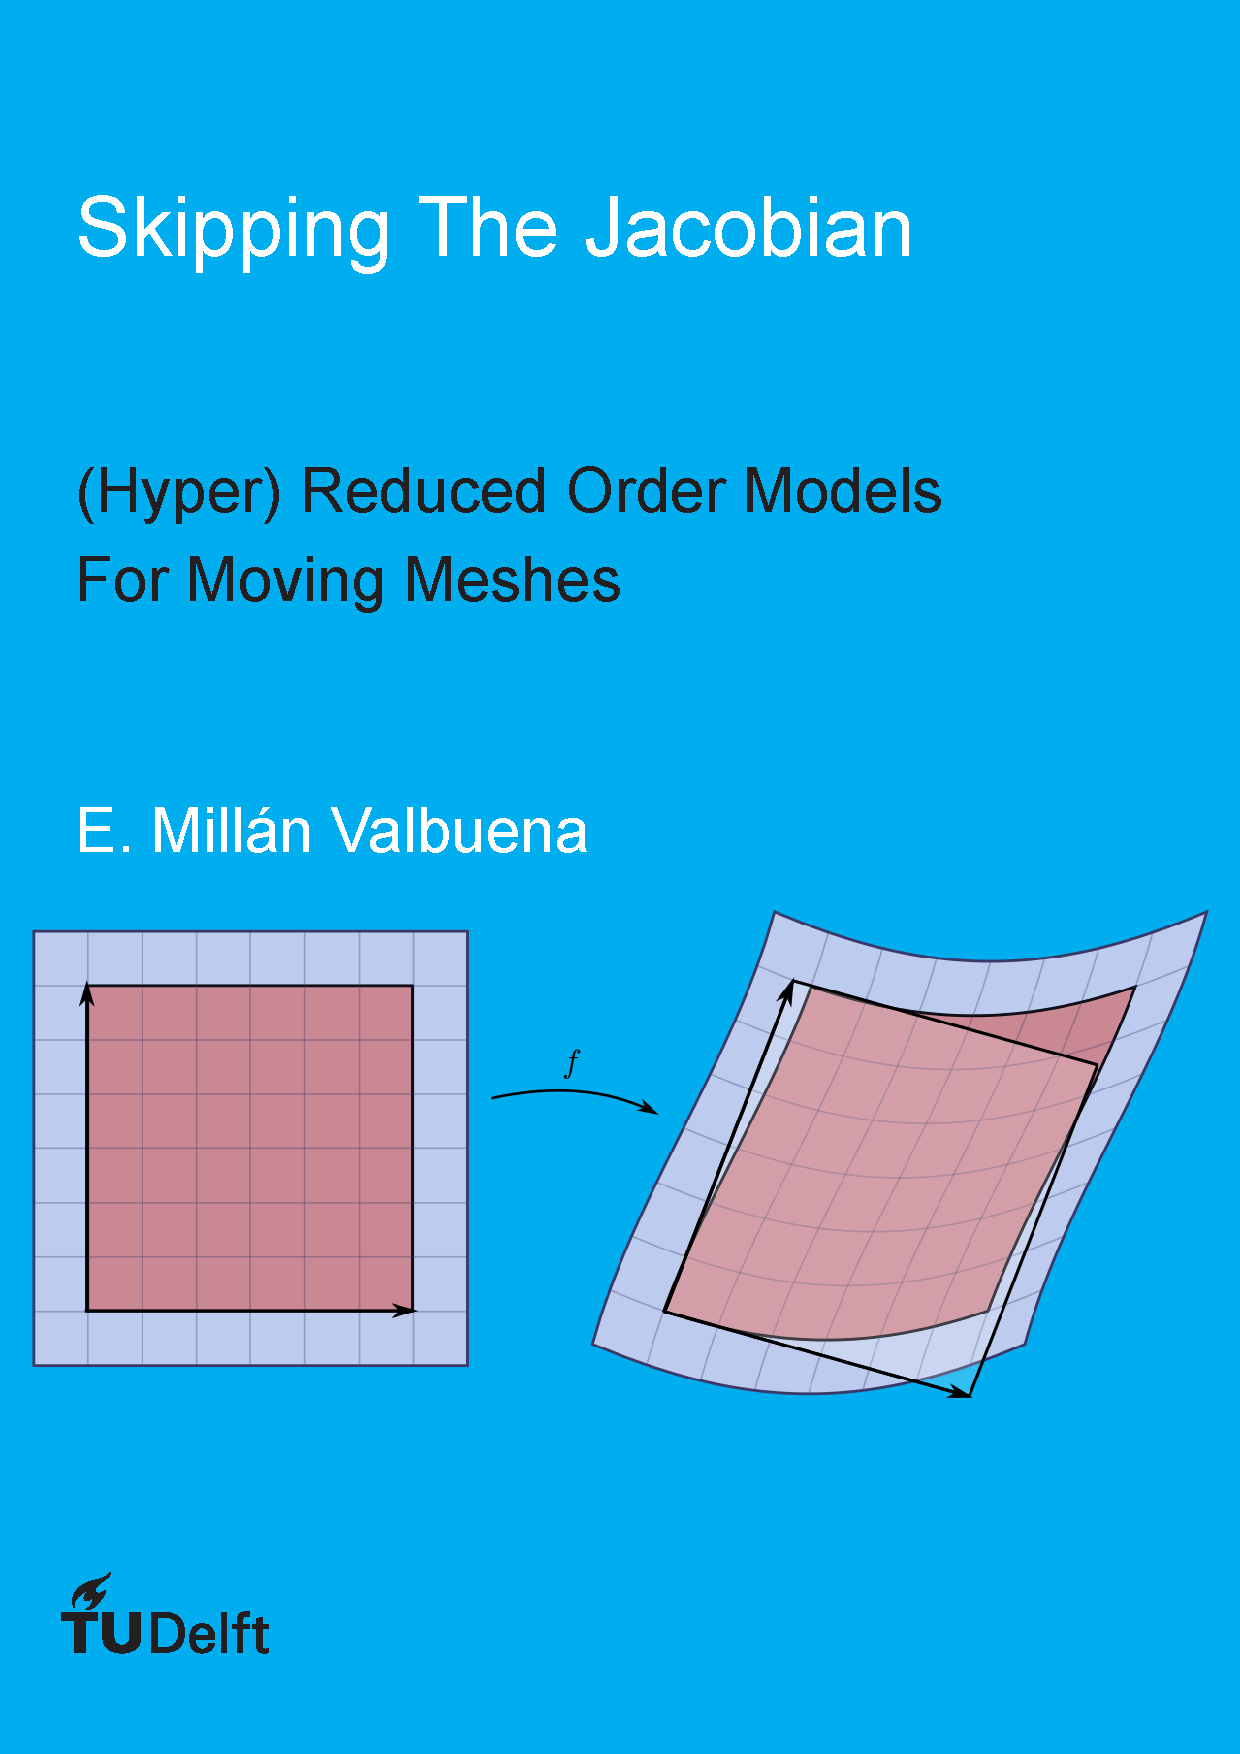
\includepdf[pages=-]{TUD_Report.pdf}

\onecolumn

% paper title
\title{Skipping The Jacobian \\[5mm] \large{(Hyper) Reduced Order Models For Moving Meshes}}

% author names 
\author{Enrique Millán Valbuena \\ \normalsize{463 426 8}
\\[5mm]

\begin{tabular}{ll}
    % Student number: & 4634268 \\
    % Project duration: & \multicolumn{2}{l}{February 1, 2021 -- December 8, 2021} \\
    % Thesis committee: & Dr.\ R.\ P.\ Dwight, & TU Delft, chair  \\
    %                   & Dr.\ S.\ J.\ Hulshoff, & TU Delft, supervisor \\
    %                   & Dr.\ ir.\ M.\ Pini PhD, & TU Delft \\[2mm]
    Dr.\ N.\ dal Santo,    & EPFL  \\
    Dr.\ S.\ J.\ Hulshoff, & TU Delft \\
    Dr.\ A. Manzoni,       & Politecnico di Milano \\
    Dr.\ A. Quarteroni,    & Politecnico di Milano \\[5mm]
\end{tabular}
% (TU Delft) 
% \\[2mm]
% S. Hulshoff 
% \\[5mm]
% (EPFL) 
% \\[2mm]
% N. Dal Santo
% \\[5mm]
% (Politecnico di Milano) 
% \\[2mm]
% A. Manzoni, A. Quarteroni
}% <-this % stops a space
        
% The report headers
\markboth{M. Sc. Aerospace Engineering, TU Delft}%do not delete next lines
{Shell \MakeLowercase{\textit{et al.}}: Bare Demo of IEEEtran.cls for IEEE Journals}

% make the title area
\maketitle

\begin{abstract}
   We present a reduced order model (ROM) for a one-dimensional nonlinear gas dynamics problem:
   the isentropic piston.
   The main body of the PDE, 
   the geometrical definition of the mesh nodes, 
   and the boundary conditions are parametrized.
   The full order model is obtained with a Galerkin finite element discretization,
   under the Arbitrary Lagrangian Eulerian formulation (ALE).
   To stabilize the system, an artificial viscosity term is included.
   The nonlinear convective term is linearized with a second-order extrapolation.
   The reduced basis to express the solution is obtained with the POD technique.
   To overcome the explicit use of the Jacobian transformation, 
   typical in the context of moving meshes,
   a system approximation technique is introduced.
   The (Matrix) Discrete Empirical Interpolation Method, (M)DEIM, allows us
   to work with a weak form defined in the physical domain 
   (and hence the physical weak formulation)
   whilst maintaining an efficient assembly of the algebraic operators, 
   despite their change with every time step.
   Two alternative methods are presented to collect and compress the snapshots 
   for the linearized solution-dependent convective term.
   Each method leads to a different offline stage.
   All in all, our approach is purely algebraic
   and the reduced model makes no use of full order structures, 
   thus achieving a perfect \textit{offline-online} split.
   A concise description of the reduction procedure is provided.
   The reduced model is certified with a posteriori error estimations obtained via model truncation.
   % Numerical examples to showcase computational costs and implementation details are designed, 
   % implemented and validated with the Manufactured Solutions Method.
\end{abstract}

\begin{IEEEkeywords}
    \centering
    finite elements, Galerkin, reduced order models, 
    moving mesh, ALE, 
    (M)DEIM, POD, SVD, 
    model truncation
\end{IEEEkeywords}

\newpage
\setcounter{tocdepth}{2}
\tableofcontents

% \newpage
% We present a Reduced Order Model (ROM) for a one-dimensional gas dynamics problem: the isentropic piston.
The PDE, the geometrical definition of the moving boundary, and the boundary conditions are parametrized.
The Full Order Model is obtained with a Galerkin Finite Element discretization,under the Arbitrary-Lagrangian formulation (ALE). An artificial viscosity term is included. The Reduced Basis is obtained with the classical POD technique.
To overcome the explicit use of the Jacobian transformation, a system approximation technique is used.
The (Matrix) Discrete Empirical Interpolation Method allows usto work with a weak form defined in the physical domainwhilst maintaining anefficient assembly for the algebraic operators.
All in all, our approach to the construction of the Reduced Order Model is purely algebraicand makes no use of Full Order structures, achieving a perfect offline-online split. A posteriori error estimators, obtained via model truncation, are used to certify the model.


\newpage
\subfile{foreword.tex}

\newpage
\twocolumn

\subfile{introduction.tex}
% \section*{Literature Review}
% \subfile{literature_review/literature.tex}

% \newpage
% \section*{Research Structure}
% \subfile{research_project/research.tex}
% \subfile{research_project/graph_layout.tex}
\newpage
\clearpage
\subfile{research_project/piston/burgers_1d_fom.tex}
\newpage
\clearpage
\subfile{research_project/piston/burgers_1d_rom.tex}
\newpage
\clearpage
\subfile{research_project/piston/burgers_1d_calibration.tex}
\newpage
\clearpage
\subfile{research_project/piston/burgers_1d_hrom.tex}
\newpage
\clearpage
\subfile{conclusions.tex}

\newpage
\clearpage
\printbibliography

\begin{appendices}
    \newpage
    \subfile{research_project/piston/piston_movement.tex}
    % \newpage
    % \clearpage
    % \subfile{research_project/piston/svd_analysis.tex}
    % \newpage
    % \clearpage
    % \subfile{research_project/piston/nonlinear_displacement.tex}
    % \newpage
    % \clearpage
    % \subfile{research_project/piston/parameter_range_selection.tex}
    \newpage
    \clearpage
    \onecolumn
    \subfile{research_project/piston/large_graphics.tex}
\end{appendices}

\end{document}